%! TEX root = **/010-main.tex
% vim: spell spelllang=en:

\subsection{Decision Trees}%
\label{sub:decision-trees}
We decided that in order to find the ideal depth of the decision tree, we had to try a range of values and pick the best performing one.

\begin{figure}[H]
    \centering
    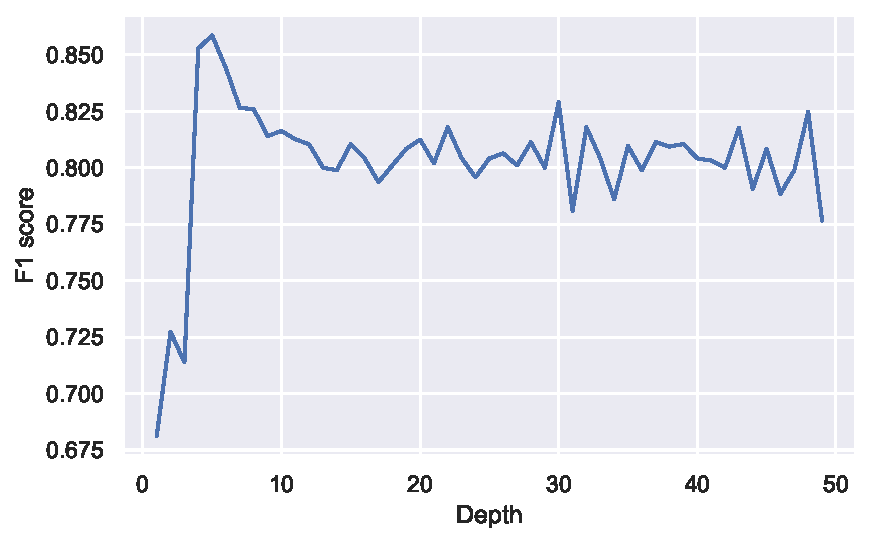
\includegraphics{decision_trees}
    \caption{Decision trees F1 Score depending on the maximum depth of the decision tree.}%
    \label{fig:decision_trees_acc}
\end{figure}

As we see, we tried all values between 1 and 50 and we found out that the best performing depth was around 5. 

The resulting tree was surprisingly simple, and we could find very good leafs, with a gini index of 0 and 300+ samples in it and also a pretty bad leaf that had a gini value of 0.5 but just 34 samples. The majority of the examples though were classified by two leafs that had a really small gini and a very big number of samples, that'd make it a pretty good classifier.

To explain in a simple way what the tree does, we could say that it first tries to find the examples that are clearly a False Positive with the rightmost branches and after that, tries to classify the remaining ones. We can understand that this behaviour is reinforced by the nature of our data, that's skewed towards the False Positive class.

\begin{landscape}
\null
\vfill
\begin{figure}[H]
    \centering
    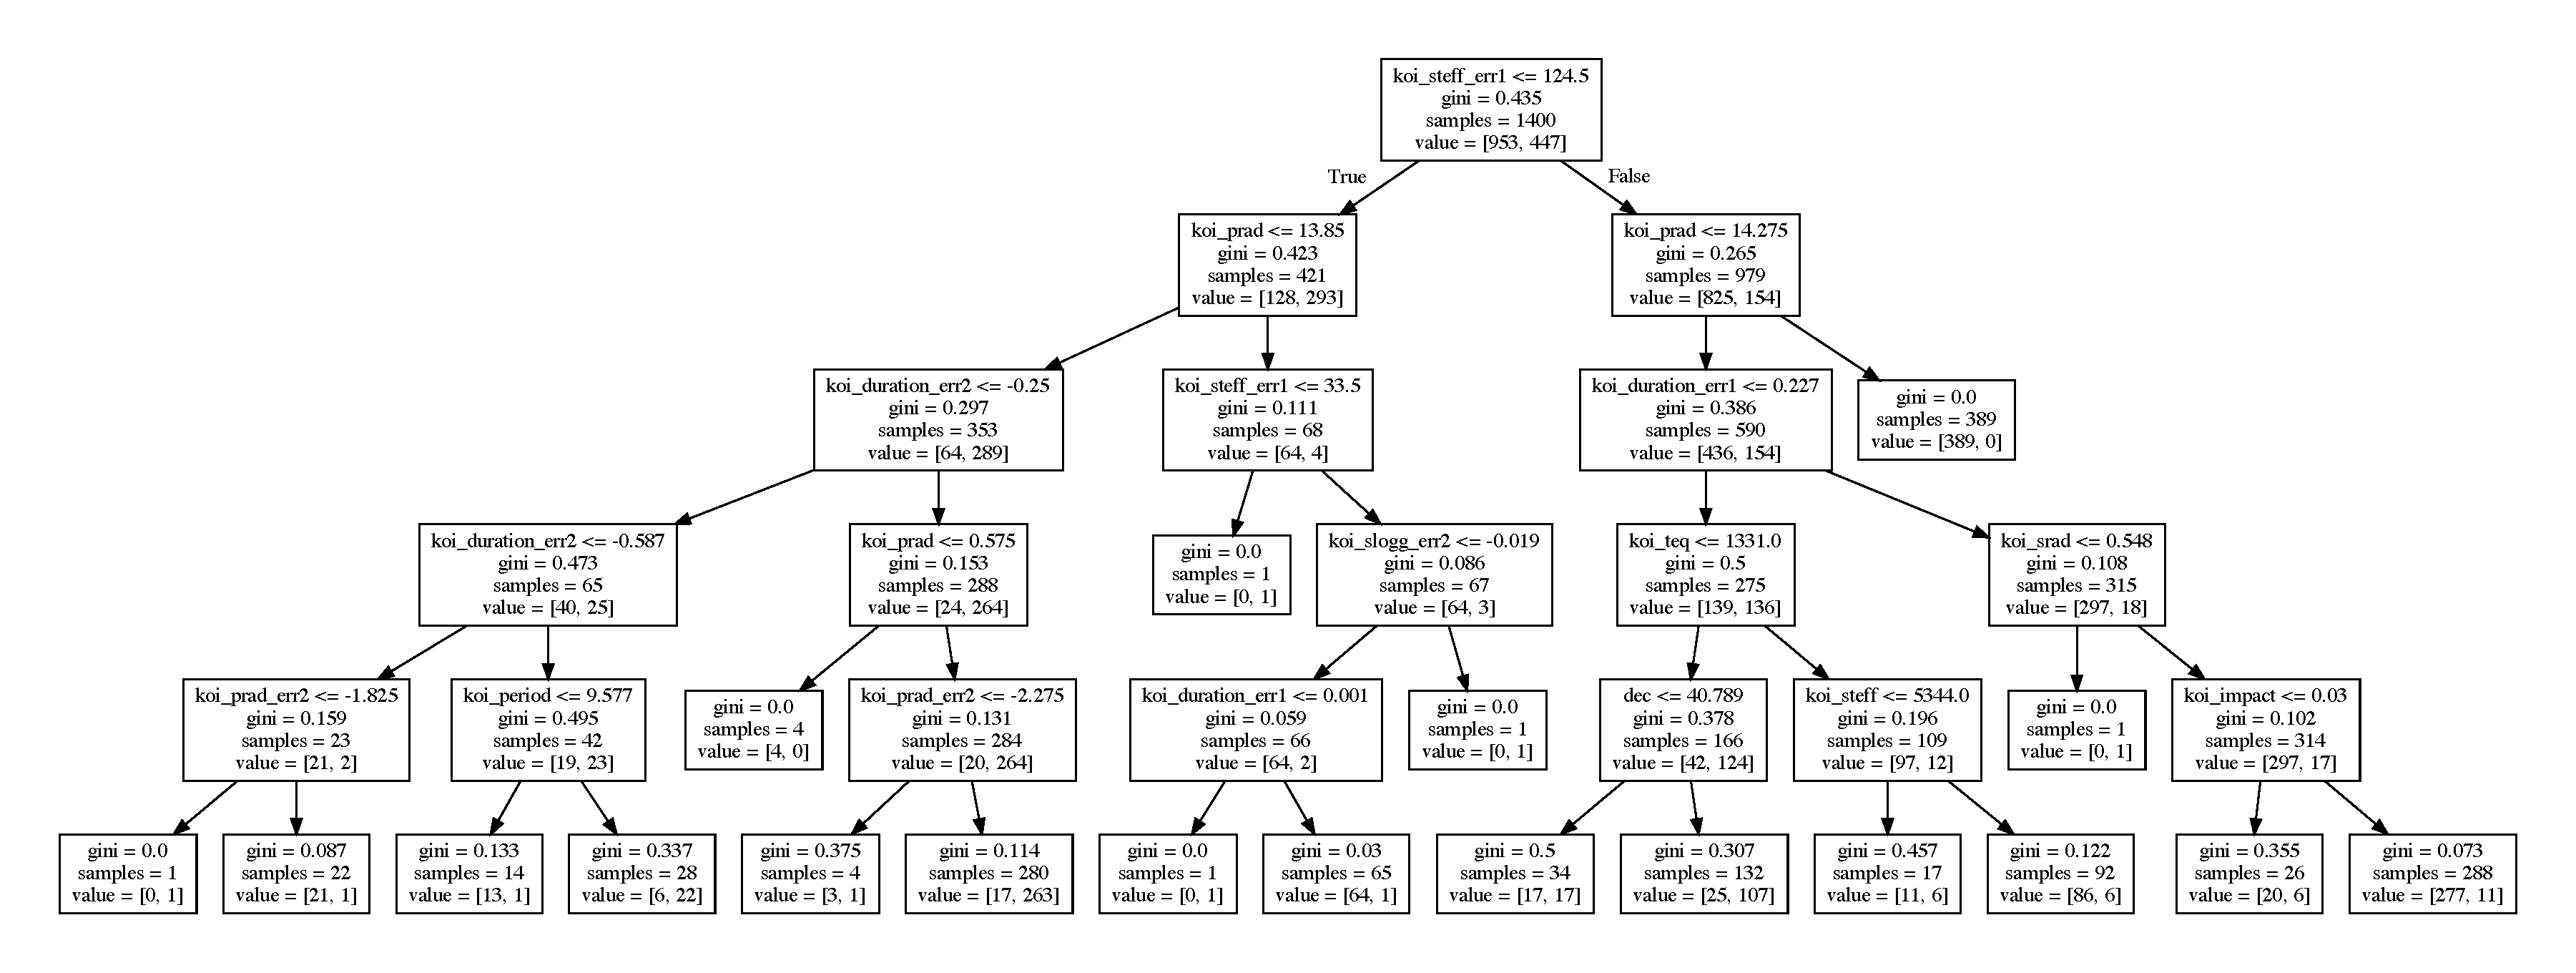
\includegraphics[width=23cm]{decision_tree}
    \caption{Our best-performing decision tree.}%
    \label{fig:decision_trees}
\end{figure}
\vfill
\null
\end{landscape}

% Discussion of choice of parameters used. Try to interpret the obtained DT using some examples of the validation set. 
% Show some of the most relevant rules.  Discuss how + and – examples are mixed in leaves in order to
% estimate the reliability of the tree.